\section{Adversarial Machine Learning}\label{sec:adversarial-machine-learning}
Deep Learning algorithms have achieved the state-of-the-art performance in many tasks. 
However, the interpretability of deep neural networks is still unsatisfactory as they work as black boxes, which means it is difficult to get intuitions from what each neuron exactly has learned. 
One of the problems of the poor interpretability is evaluating the robustness of deep neural networks. 


Adversarial Machine Learning is a collection of techniques to train neural networks on how to spot intentionally misleading data or behaviors. 
This differs from the standard classification problem in machine learning, since the goal is not just to spot “bad” inputs, but preemptively locate vulnerabilities and craft more flexible learning algorithms.

The objective of an adversary
could be to attempt to manipulate either the data collection or
the data processing in order to corrupt the target model, thus
tampering the original output. 

Unlike traditional cybersecurity
attacks, these weaknesses are not due to mistakes made by programmers or users. They are
just shortcomings of the current state-of-the-art
methods. Put more bluntly, the algorithms that
cause AI systems to work so well are imperfect,
and their systematic limitations create opportunities for adversaries to attack. At least for the foreseeable future, this is just
a fact of mathematical life \cite{Comiter2019AttackingAI}.

Two main types of AI attacks can be defined according to the time at which the attack happens \cite{journals/corr/abs-1810-00069}:
\begin{itemize}
    \item \textbf{Adversarial Attacks (Evasion)}: this is the most common type of attack in
    the adversarial setting. The adversary tries to evade the system by adjusting malicious samples during the testing phase. This
    setting does not assume any influence over the training data.
    In Figure \ref{fig:2_2_evasion} is depicted how adding an imperceptible and carefully constructed noise to the input originally recognized as “panda” with 57.7\% confidence, we can change
    the classification output given by the same neural network toward another target (in the example “gibbon” with 99.3\% confidence).
    \item \textbf{Data Poisoning Attacks}: This type of attack, known as contamination of the training data, is carried out at training phase of
    the machine learning model. An adversary tries to inject
    skilfully crafted samples to poison the system in order to
    compromise the entire learning process. The Figure \ref{fig:2_2_data_poisoning} shows as in normal machine learning (left), the learning algorithm extracts
    patterns from a dataset, and the “learned” knowledge is stored in the machine
    learning model---the brain of the system. In a poisoning attack (right), the
    attacker changes the training data to poison the learned model. 
\end{itemize}

\begin{figure}[H]
    \begin{subfigure}{0.45\textwidth}
      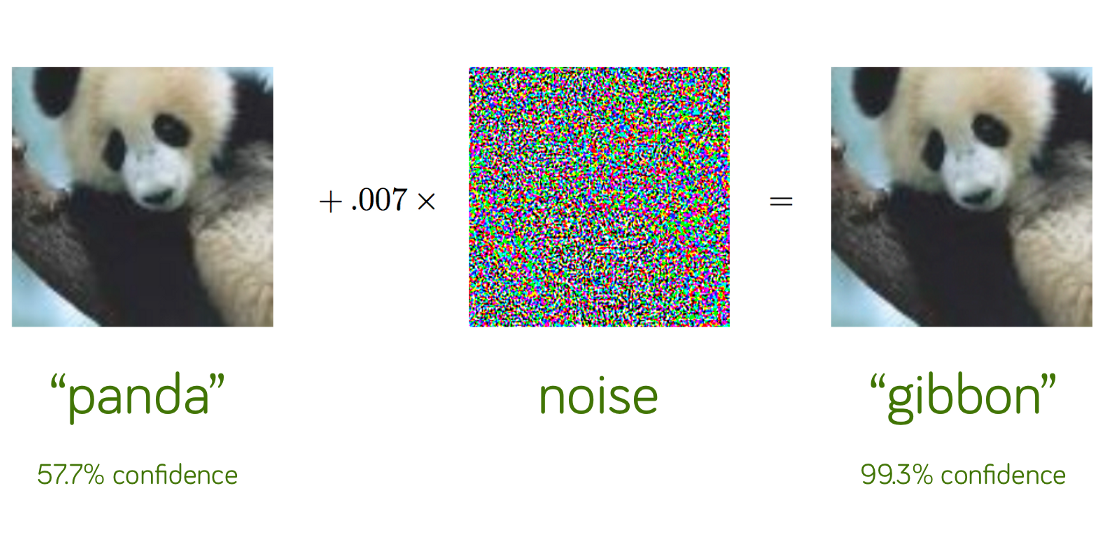
\includegraphics[width=\linewidth]{images/2_2_evasion.png}
      \caption{Evasion attack on image classification \cite{szegedy2013intriguing}} \label{fig:2_2_evasion}
    \end{subfigure}%
    \hspace*{\fill}   % maximize separation between the subfigures
    \begin{subfigure}{0.45\textwidth}
      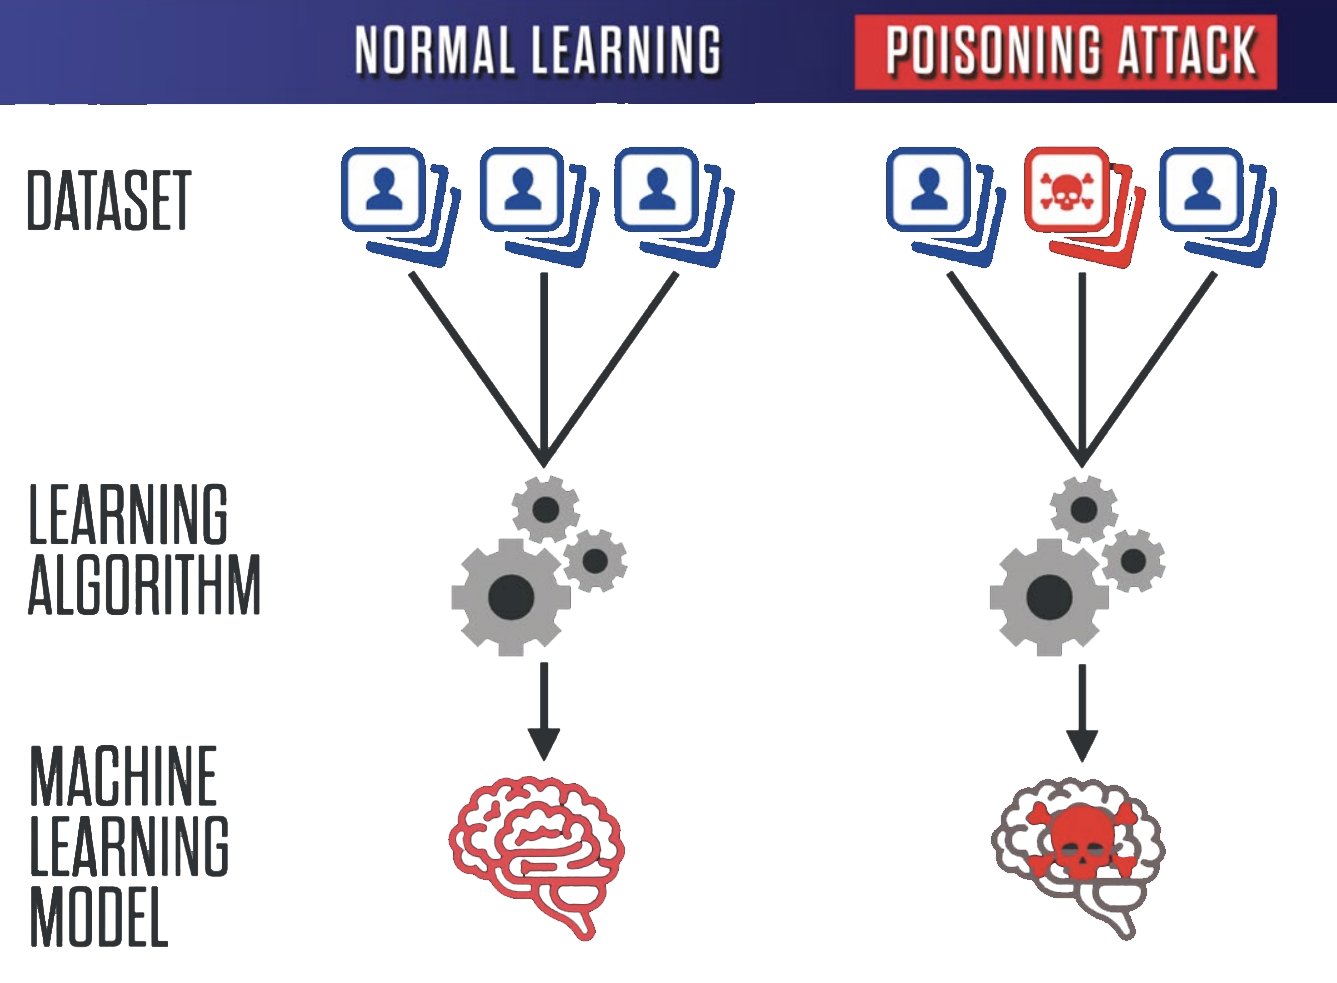
\includegraphics[width=\linewidth]{images/2_2_data_poisoning.png}
      \caption{Poisoning attack on training data \cite{Comiter2019AttackingAI}} \label{fig:2_2_data_poisoning}
    \end{subfigure}
  \caption{Examples of Artificial Intelligence Attacks} \label{fig:2_2_adversarial_attacks}
  \end{figure}

In this thesis, we will focus on the first type of attack: Adversarial Attacks.
Over the past few years, researchers \cite{goodfellow2014explaining, szegedy2013intriguing} used small unperceivable perturbations to evaluate the robustness of deep neural networks and found that they are not robust to these perturbations. 

%**************************************************************
\subsection{Adversarial examples}\label{subsec:adversarial-attacks}

Szegedy et al. \cite{szegedy2013intriguing} first evaluated the state-of-the-art deep neural networks used for image classification with small generated perturbations on the input images.
They found that the image classifiers were fooled with high probability, but human judgment is not affected. The perturbed image pixels were named \emph{adversarial examples} and this notation is later used to denote all kinds of perturbed samples in a general manner.
Formally, adversarial example $x^\prime$ is an example created via worst-case perturbation of the input to a deep learning model. An ideal deep neural network would still assign correct class $y$ (in the case of classification task) to $x^\prime$, 
while a victim deep neural network would have high confidence on wrong prediction of $x^\prime$. $x^\prime$ can be formalized as:
\begin{equation}
    \begin{array}{l}
    x^\prime = x + \eta, \quad f(x)=y, \quad x \in X,\\
    f(x^\prime) \neq y, \\
    \text{or} \quad f(x^\prime) = y^\prime, \quad y \neq y^\prime
    \end{array}
\end{equation}
where $\eta$ is the worst-case perturbation. The goal of the adversarial attack can be deviating the label to incorrect one ($f(x^\prime) \neq y$) or specified one ($f(x^\prime) = y^\prime$) \cite{journals/tist/ZhangSAL20}.

%**************************************************************
\subsection[Paradigm shift]{Paradigm shift: from CV to NLP}\label{subsec:paradigm-shift}
Adversarial examples were first proposed for attacking DNNs for object recognition in the \acrfull{cv} community.
The former work on this field by Szegedy et. al. \cite{szegedy2013intriguing}  was based on L-BFGS, but despite the effectiveness of the method, it was computationally expensive and impractical.
Goodfellow et al. \cite{goodfellow2014explaining} proposed a \acrfull{fsgm} that popularized this research topic. It is a simplification of the L-BFGS method since it adds a small perturbation to the input of a model, which is computed by taking the sign of the gradient of the loss function with respect to the input.
Most follow-up research was based on optimization methods (eg. JSMA \cite{journals/corr/PapernotMJFCS15}, DeepFool \cite{journals/corr/Moosavi-Dezfooli15}, C\&W \cite{journals/corr/CarliniW16a}) or leveraging \acrfull{gan} to generate adversaries \cite{journals/corr/abs-1710-11342}.

As shown in Figure \ref{fig:2_2_adversarial_trend}, adversarial technology has attracted attention and has developed rapidly. Based on the paper list\footnote{\url{https://nicholas.carlini.com/writing/2019/all-adversarial-example-papers.html}} collected by Carlini, the chart counts
the number of publications related to adversarial in the CV and NLP fields. Compared with studies in the CV field, the publications in the NLP domain are far fewer. However, due to the wide application of NLP technology in text classification, sentiment analysis, text question-answering, neural machine translation, text generation and other tasks, as well as the continuous deepening of adversarial attack and defence technologies, textual adversarial technology has gradually gained researchers' attention.

\begin{figure}
    \centering
    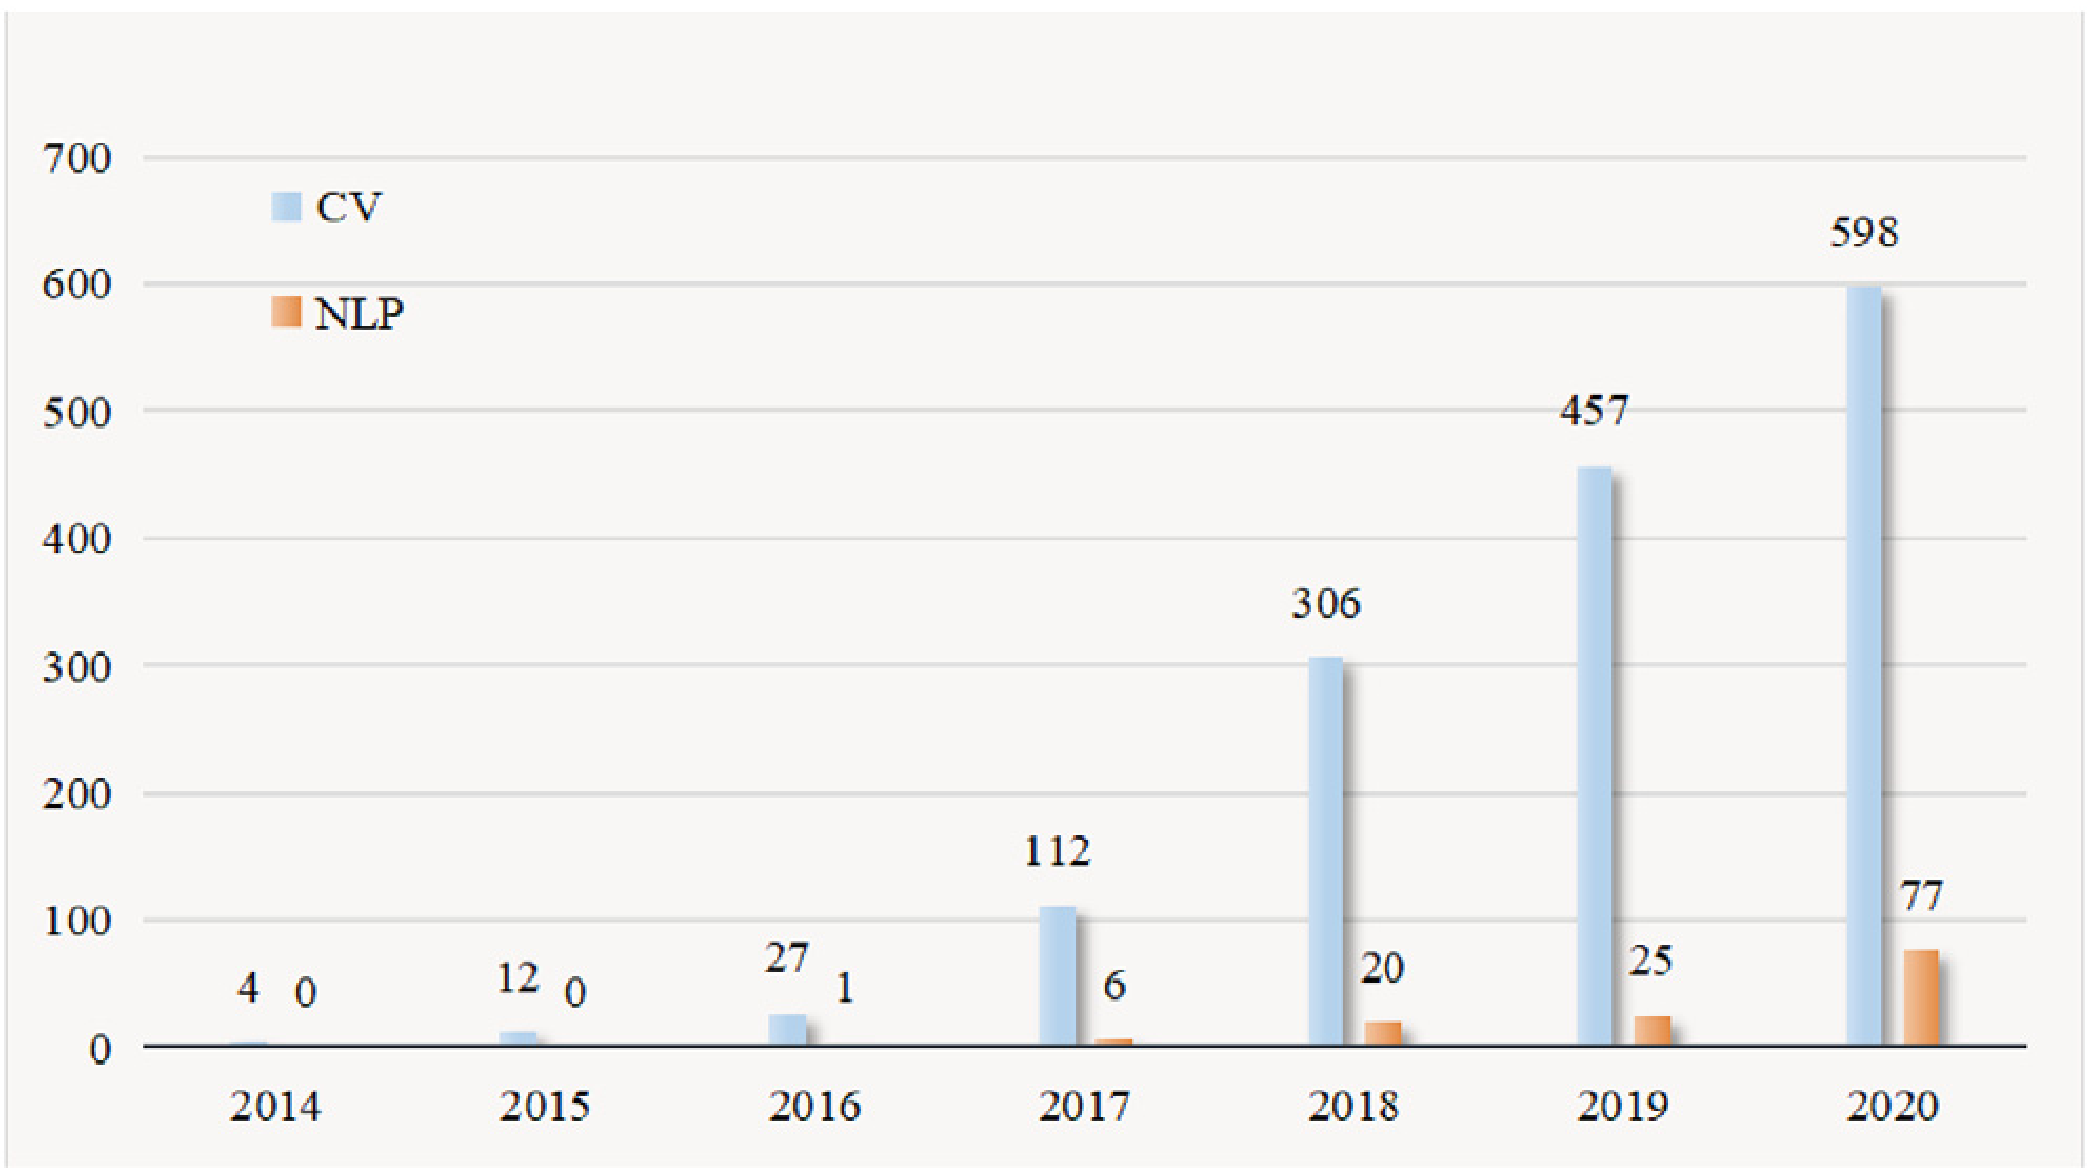
\includegraphics[width=0.8\linewidth]{images/2_2_papers.png}
    \caption{Adversarial technology trend in CV and NLP fields \cite{QIU2022278}}
    \label{fig:2_2_adversarial_trend}
\end{figure}

Papernot et al. \cite{journals/corr/PapernotMSH16} are the first to investigate adversarial attacks
on texts. Inspired by the idea of generating adversarial images, they crafted adversarial texts through the forward derivative associated with texts' embeddings, by modifying characters or words in original texts.


\subsubsection{Particularities of adversarial text}\label{subsubsec:particularities-of-adversarial-text}

Publications related to adversarial technology in the NLP field are far less than those in the CV field.
The reason is that three extra constraints need to be considered when generating textual adversarial examples. Specifically:
\begin{itemize}
    \item \textbf{Discrete}: Unlike images represented by continuous pixel values, the symbolic text is discrete. Therefore, finding appropriate perturbations is critical to efficient textual adversarial example generation. 
                             It is hard to define the perturbations on texts. Carefully designed variants or distance measurements for textual perturbations are required.
    \item \textbf{Perceivable}: The well-performed adversarial image generation method is based on the premise that a few pixel value changes in an image are invisible to human eyes. However, a slight modification of a character or word is easily realized by human eyes and spelling checkers. Hence, finding textual adversarial examples that are hard to be observed by human eyes is vital for successful adversarial attacks.
    \item \textbf{Semantic}: Compared with images whose overall semantics do not change when changing a few pixel values, the semantics of a text could be altered by even replacing or adding a character, violating the principle that adversarial examples are perceivable to humans. Therefore, keeping the semantics consistent is the key to crafting influential adversarial texts.
\end{itemize}

These differences make it extraordinarily difficult for
researchers to employ methods dealing with images to adversarial attacks. Moreover, one of the first tasks of NLP
models is to work on real data to check their generalization ability. Although adversarial attacks are a practical approach to evaluate robustness, most of them have the problem of being task-specific, not being well generalized, and not presenting comprehensive guidelines for evaluating system robustness.

%**************************************************************
\subsection{Taxonomy of textual adversarial attacks}\label{subsec:taxonomy-textual-adversarial-attacks}

Textual adversarial attack methods can be categorized according different criteria. In this section, we will introduce the taxonomy of textual adversarial attacks based on model access, adversarial goal, semantic granularity and attack strategy, as shown in Figure \ref{fig:2_2_taxonomy}.

\begin{figure}
    \centering
    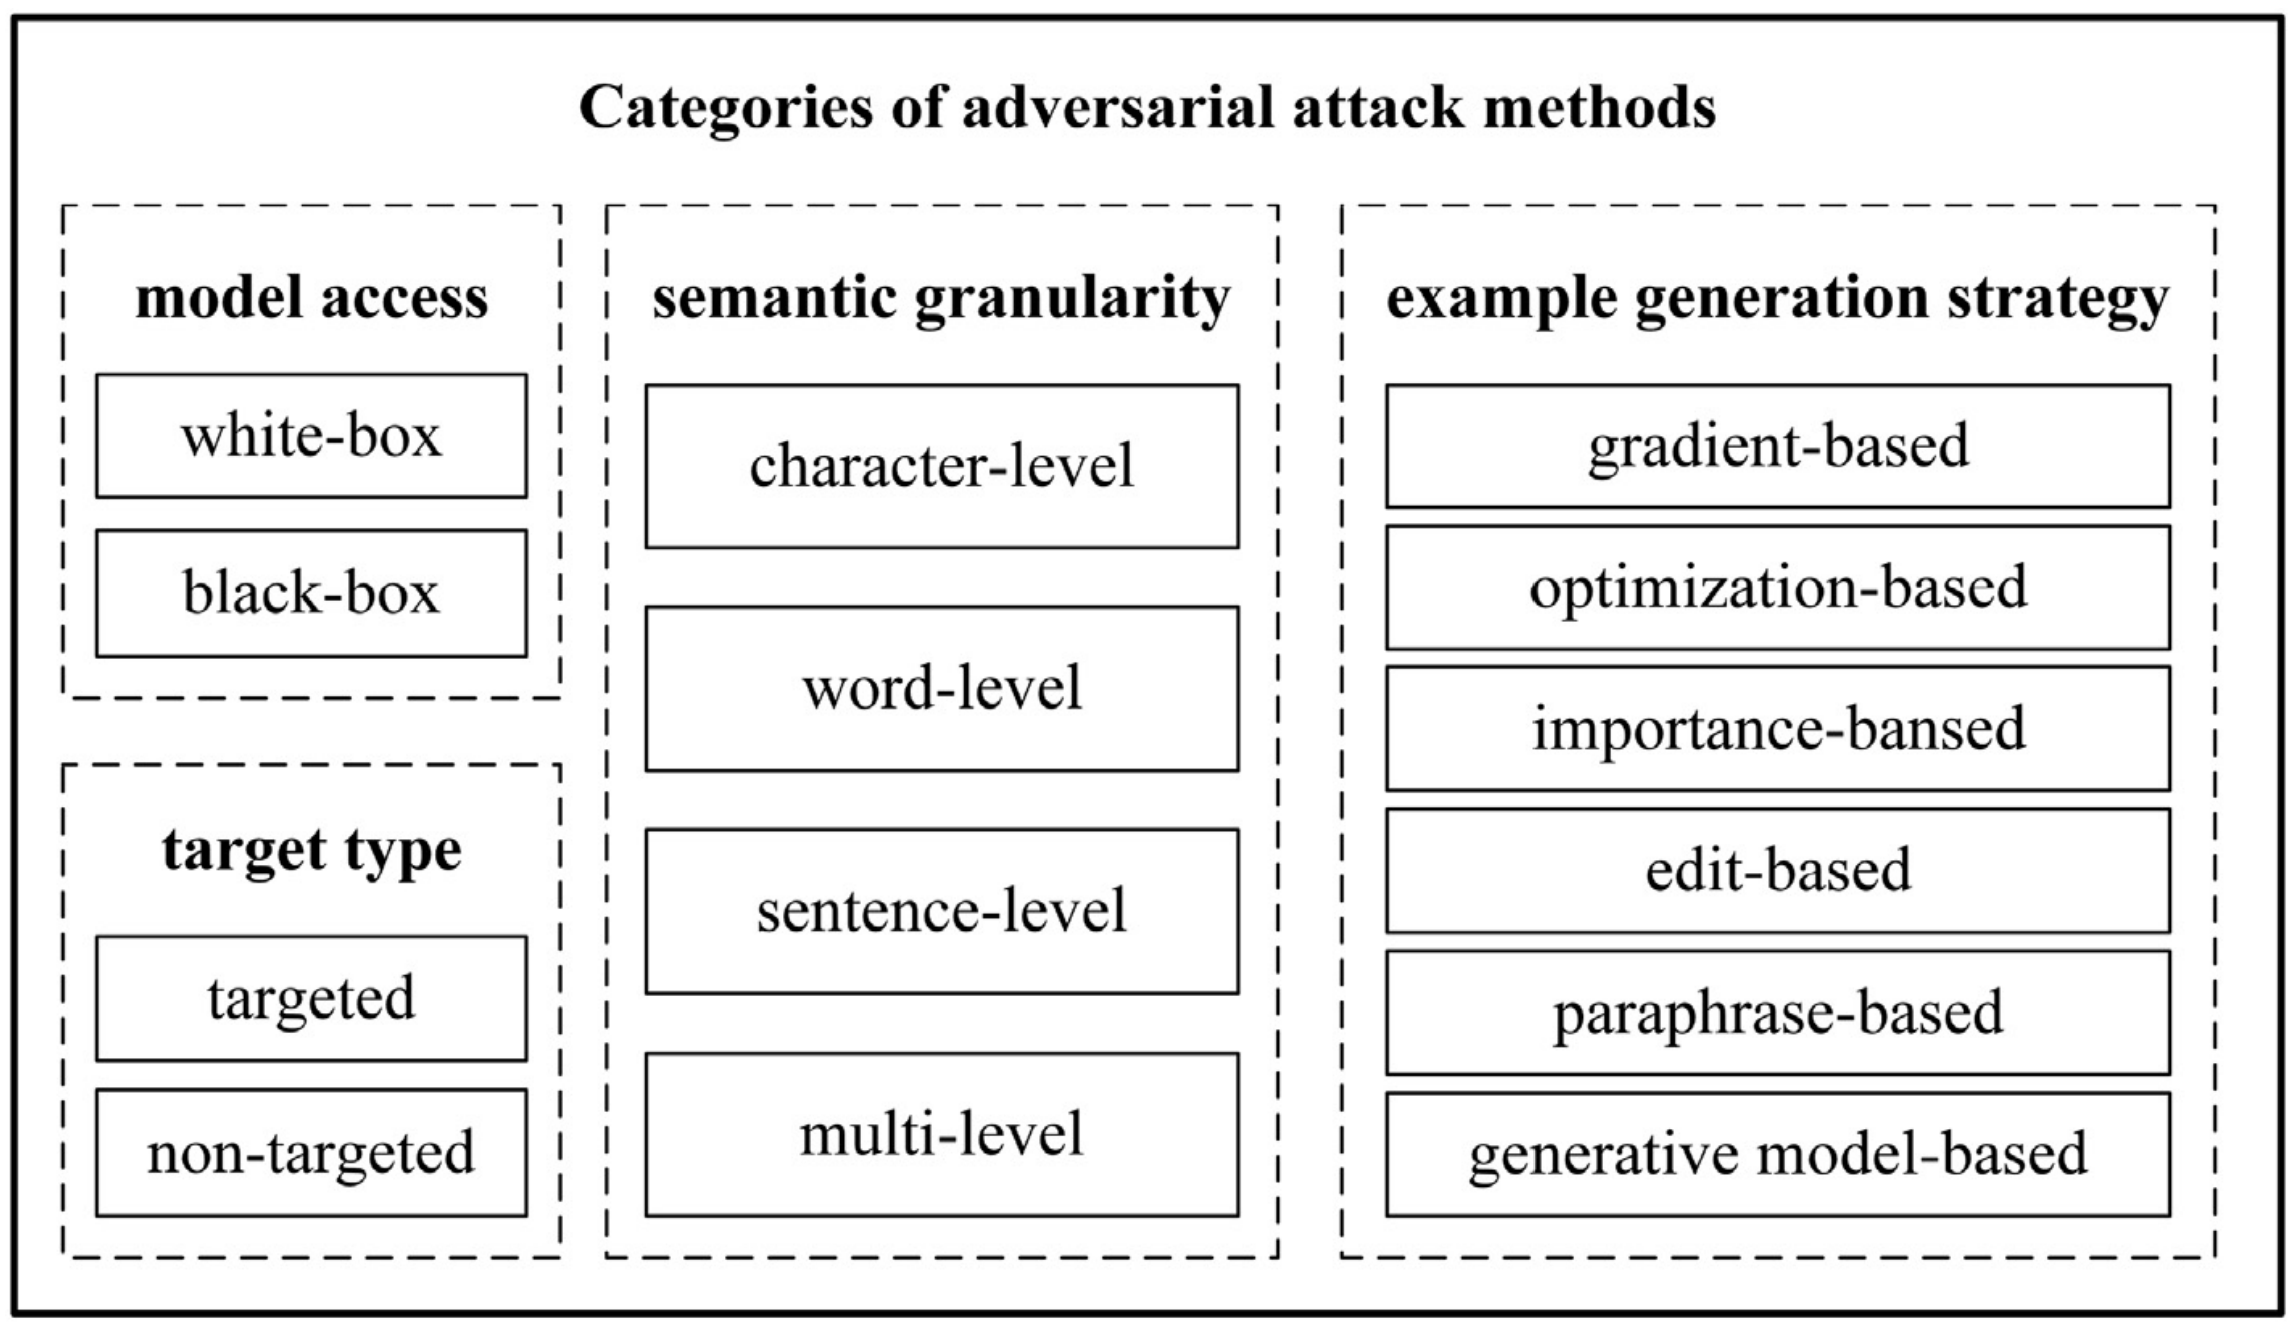
\includegraphics[width=0.8\linewidth]{images/2_2_taxonomy.png}
    \caption{Categorization of textual adversarial attack methods \cite{QIU2022278}}
    \label{fig:2_2_taxonomy}
\end{figure}

%-------------------------------------------------------------
\subsubsection{Model access}\label{subsubsec:model-access}

Adversarial attacks at the testing time do not tamper with the targeted model but rather forces it to produce incorrect outputs. 
The effectiveness of such attacks
is determined mainly by the amount of information available to the adversary about the model.
Testing phase attacks can be broadly classified into either \emph{white-box} or \emph{black-box} attacks \cite{journals/corr/abs-1810-00069}.

\textbf{White-Box Attacks}. In white-box attack on a machine learning model, an adversary has total
knowledge about the model used for classification (e.g., type of neural network along with number of layers). The attacker has information about the algorithm used in training (e.g.
gradient-descent optimization) and can access the training data distribution. He also knows the
parameters of the fully trained model architecture. The adversary utilizes available information
to identify the feature space where the model may be vulnerable, for which the model has
a high error rate. Then the model is exploited by altering an input using adversarial example
crafting method.

\textbf{Black-Box Attacks}. Black-box attack, on the contrary, assumes no knowledge about the model
and uses information about the settings or past inputs to analyse the vulnerability of the model.
For example, in an oracle attack, the adversary exploits a model by providing a series of carefully
crafted inputs and observing outputs.  For example, to identify meaningful words in given texts, works in \cite{journals/corr/SamantaM17, conf/acl/RenDHC19, journals/corr/abs-1907-11932} computed the probability change value, word saliency, and classification probability by using the victim model's output.


%-------------------------------------------------------------
\subsubsection{Adversarial goal}\label{subsubsec:adversarial-goal}

According to the attack purpose of an adversary, adversarial
attack methods are categorized into targeted and non-targeted attacks \cite{QIU2022278}.

\textbf{Non-targeted attack}. The adversary hopes to generate an adversarial example $x^\prime$ that makes the victim model $f$ produce a wrong output $f(x^\prime) \neq y$, where $y$ is the correct label of the input $x$. Since there is no limit on the target's wrong output, this kind of attack is more frequently employed.

\textbf{Targeted attack}. In this scenario, the adversary intends to generate adversarial examples that make victim models output a specified wrong prediction. More specifically, the adversary hopes that the generated example $x^\prime$ to cause the victim model $f$ outputting $t=f(x^\prime)$, where $t$ is the output specified by the adversary.

%-------------------------------------------------------------
\subsubsection{Attack strategy}\label{subsubsec:attack-strategy}

According to different strategies in the adversarial example generation process, Shilin Qiu et al. \cite{QIU2022278} divide adversarial attacks into six types: gradient-based, optimization-based, importance-based, edit-based, paraphrase-based, and generative model-based methods. Among them, strategies like the gradient-based method are evolved from adversarial image generation methods, and the implementation process of these attacks is usually relatively straightforward. While other methods like the optimization-based and edit-based methods are proposed for discrete data, they generally show better performance in maintaining semantic consistency and grammatical correctness; however, they have enormous difficulty when designing well-turned algorithms.

\textbf{Gradient-based}. These methods calculate the forward derivative to the input and obtain adversarial perturbations by gradient backpropagation. Therefore, the vectorization for text needs to be implemented at first.

\textbf{Optimization-based}. It regards the adversarial example generation as a minimax optimization problem, i.e., maximizing the victim model's prediction error while the difference between the adversarial example and the original one is within an acceptable range. Currently, researchers craft adversarial texts essentially based on evolutionary algorithms, such as the \acrshort{ga} and \acrshort{pso}.

\textbf{Importance-based}. This means that which object is to be modified and how to modify it are determined by each object's importance related to the victim model. Since the more critical the changed word is, the easier it is to change the prediction of the victim model, even if the change is small enough. The adversarial example generated by this strategy generally maintains semantic consistency, grammatical, and syntactic correctness well.

\textbf{Edit-based}. It crafts adversarial examples by operations like inserting, removing, and swapping characters, words, or sentences. These editing operations are also used in other approaches, such as gradient-based, optimization-based, and importance-based methods. Therefore, the edit-based method refers to attacks that utilize the above editing operations but do not use the gradient information, optimization algorithm, or item importance.

\textbf{Paraphrase-based}. The adversary takes the paraphrase of a sentence as its adversarial example. In the paraphrase generation process, the adversary introduces different extra conditions to fool the victim model without affecting human judgment. The sentence-level attacks commonly use these approaches.

\textbf{Generative model-based}. This method uses the generative model like the GAN and encoder-decoder model to generate adversarial texts, and is frequently used in sentence-level attacks. Since there are gradient back propagations when training the generative model or crafting adversarial examples, these methods are usually combined with other techniques, such as \acrshort{rl}.

%-------------------------------------------------------------
\subsubsection{Semantic granularity}\label{subsubsec:semantic-granularity}

Since the text is discrete, classifying adversarial attacks according to semantic granularity is more intuitive than NLP tasks or black/white-box scenarios.
Thus, Huq et al. \cite{https://doi.org/10.48550/arxiv.2005.14108} divided textual adversarial attacks into four categories: character-level, word-level, sentence-level, and multi-level attack.

\textbf{Character-Level Attack}. Individual characters in this attack are either modified with new characters, special characters, and numbers. These are either added to the text, swapped with a neighbour, removed from the word, or flipped.

\textbf{Word-Level Attack}. In this attacks words from the texts are changed with their synonyms, antonyms, or changed to appear as a typing mistake or removed completely.

\textbf{Sentence-Level Attack}. This attack inserts extra distractor sentences, generates the paraphrase, or modifies the original sentence structure to fool the victim model.

\textbf{Multi-Level Attack}. Attacks which can be used in a combination of character, word, and sentence level are called multi-level attacks.

%**************************************************************
\subsection{Adversarial attack methods from literature}\label{subsec:aam-from-literature}

Several adversarial attack methods have been proposed in the literature. In this section, we present a brief overview of the most popular ones, listed in Table \ref{tab:attack-methods}.

Those methods are categorized according to the classification defined in Sec. \ref{subsubsec:semantic-granularity}:
1 character-level attack (DeepWordBug \cite{journals/corr/abs-1801-04354}), 4 word-level attacks (Probabilistic Weighted Word Saliency (PWWS) \cite{conf/acl/RenDHC19}, TextFooler \cite{journals/corr/abs-1907-11932}, BERT-based attack \cite{conf/emnlp/LiMGXQ20} and Semese-PSO \cite{conf/acl/ZangQYLZLS20}), 2 sentence-level attacks (Synthetically Controlled Paraphrase Networks (SCPNs \cite{conf/naacl/IyyerWGZ18}), and GAN-based attack \cite{journals/corr/abs-1710-11342}), and 1 multi-level attack (TextBugger \cite{conf/ndss/LiJDLW19}).

DeepWordBug determines top critical tokens and modify them by character-level transformations introducing typos. 
PWWS is a synonym-based substitution method that makes use of the word saliency and classification probability.
TextFooler identifies important words, and replaces them with the most semantically similar and grammatically correct substitutes.
BERT-based attack finds the vulnerable words for the target model and replaces them with candidates from a pre-trained BERT model.
Semese-PSO reduces search space by a sememe-based word replacement method, searching for adversarial examples through the PSO algorithm in the reduced search space.
SCPNs generates adversarial examples by paraphrasing the original sentence using an encoder-decoder model.
GAN-based attack generates adversarial examples using iterative stochastic search and hybrid shrinking search. The framework consists of a GAN and a converter.
TextBugger generates character-level and word-level adversarial texts according to the importance in black-box and white-box scenarios.

\begin{table}[h]
  \footnotesize
  \centering
  \begin{tabular}{|c||c|c|c|c|}
    \hline
    Method & Granularity & Strategy & Model access & Attack goal \\
    \hline \hline
    DeepWordBug & Character-level & Importance-based & Black-box & Non-targeted \\ 
    
    PWWS & Word-level & Importance-based & Black-box & Non-targeted \\
    
    TextFooler & Word-level & Importance-based & Black-box & Non-targeted \\
    
    BERT-based & Word-level & Importance-based & Black-box & Non-targeted \\
    
    Semese-PSO & Word-level & Optimization-based & Black-box & Non-targeted \\
    
    SCPNs & Sentence-level & Paraphrase-based & Black-box & Non-targeted \\
    
    GAN-based & Sentence-level & Generative model-based & Black-box & Non-targeted \\
    
    TextBugger & Multi-level & Importance-based & Black/White-box & Non-targeted \\
    \hline
  \end{tabular}
  \caption{Several adversarial attack methods from literature}
\label{tab:attack-methods}
\end{table}


To give readers a more intuitive understanding of these attack
methods, in Figure \ref{fig:2_2_adversarial_examples} are showed adversarial examples generated by each method. 
The original examples are two randomly selected from the \acrfull{sst} dataset, and both of them are correctly classified as Positive by the pre-trained BERT model for sentiment analysis.

From the perspective of example quality, character-level attack
methods maintain the semantics of original texts well. However, they are easily detected by human eyes or spelling check tools.
In contrast, word-level attacks compensate for the vulnerability of adversarial examples to detection but affect the semantics of the text to some extent.
sentence-level attacks enhance the diversity of generated examples. However, it is clear to see that these adversarial examples crafted by sentence-level SCPNs and GAN-based methods are very different from the original ones in both semantics and readability. 

\begin{figure}[H]
  \centering
  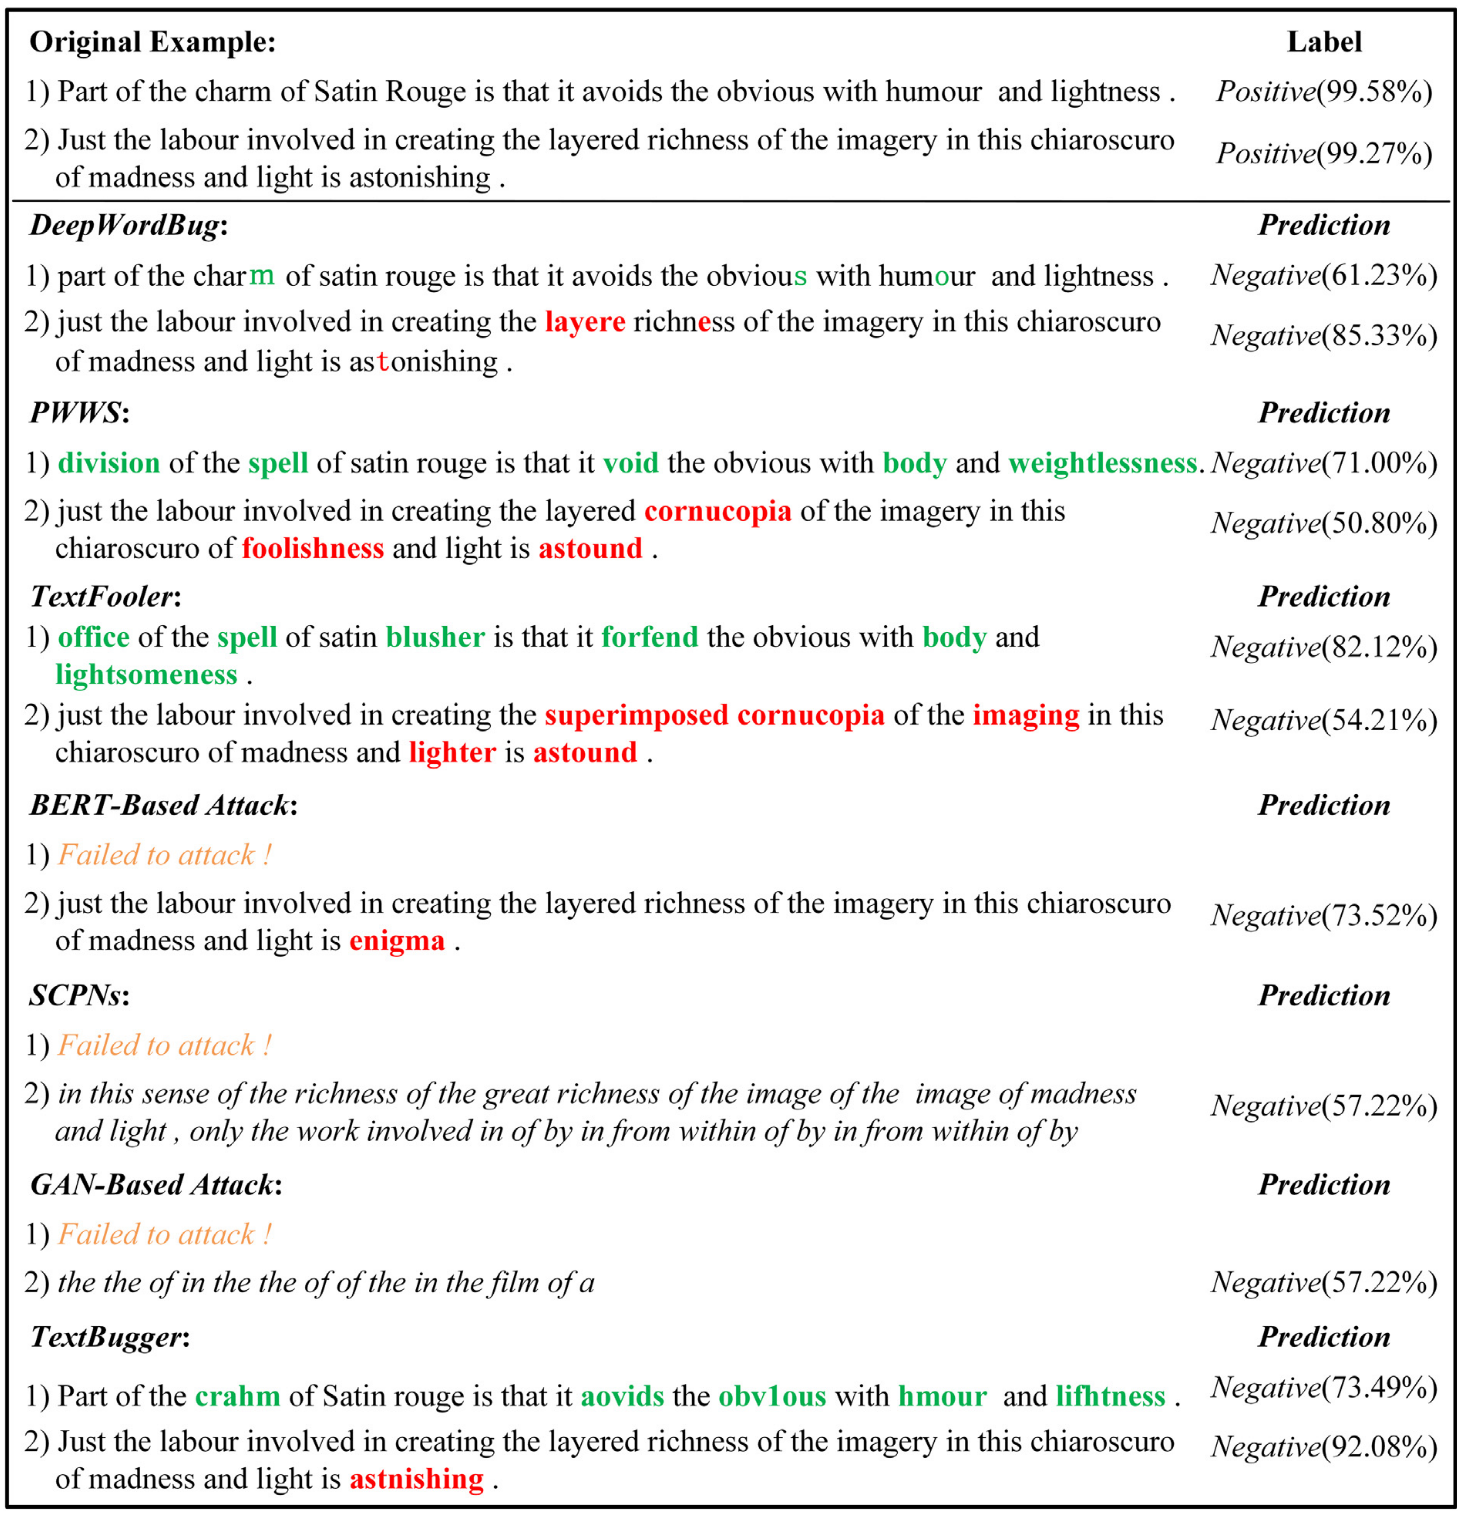
\includegraphics[width=0.9\linewidth]{images/2_2_adversarial_examples.png}
  \caption{Adversarial examples generated by different methods \cite{QIU2022278}}
  \label{fig:2_2_adversarial_examples}
\end{figure}

For comparing the attack performance of the above methods, Shilin Qiu et. al. \cite{QIU2022278} randomly selected 5000 examples from the SST dataset to generate corresponding adversarial texts and attack the selected victim model using the above methods. 
The end goal of the attack algorithms is to trick
the model to make wrong prediction by manipulating the input. So the \gls{attack-success-rate} of an evasion algorithm is defined as
the percentage of wrong prediction by the victim model on the adversarial examples \cite{conf/acl-wnlp/TsaiYC19}.
Table \ref{tab:2_2_attack-performance} shows the result.
In terms of attack success rate, TextBugger is the highest, and its execution time is also relatively low. The reason might be that TextBugger uses the Jacobian matrix to calculate the importance of each word at once. In comparison, the average model queries of sentence-level methods (SCPNs and GAN-based method) are the lowest, but their attack success rates are not satisfactory. As mentioned above, the differences between the adversarial examples generated by sentence-level methods and the original ones are relatively huge, so researchers should focus on maintaining the semantic consistency and imperceptibility of texts for sentence-level methods.
Focusing on word-level attacks, the model query are comparatively numerous. However, TextFooler and BERT-based attack have a relatively highest attack success rate and a low execution time. 

Since this thesis focuses on the word-level attack, we will introduce the details of TextFooler and BERT-based attack in the following sections and use them as the baseline for our proposed method.

\begin{table}[h]
  \footnotesize
  \centering
  \begin{tabular}{|c||c|c|c|}
    \hline
    Method & Attack  & Average Model  & Average Running \\
           & Success Rate & Queries (times) & Time (seconds) \\
    \hline \hline
    DeepWordBug & 59.46\% & 23.626 & 0.000439 \\
   
    PWWS & 75.74\% & 117.82 & 0.002190 \\
   
    TextFooler & 74.86\% & 61.68 & 0.053360 \\
   
    BERT-based & 88.44\% & 61.94 & 0.036131 \\
   
    SCPNs & 75.66\% & 11.75 & 2.366100 \\
   
    GAN-based & 42.06\% & 2.42 & 0.009495 \\
   
    TextBugger & 90.54\% & 48.79 & 0.001722 \\
    \hline
  \end{tabular}
  \caption{Comparison of Adversarial Attacks Performance \cite{QIU2022278}}
\label{tab:2_2_attack-performance}
\end{table}


%--------------------------------------------------------------
\subsubsection{TextFooler}\label{subsubsec:textfooler}

TextFooler \cite{journals/corr/abs-1907-11932} is  a word-level attack in the black-box setting designed to evade two fundamental natural language tasks, text classification and textual entailment. 

For generating semantics-preserving texts with minimum modifications, it uses an importance-based strategy. First, a selection mechanism is performed to choose the words that most significantly influence the final prediction results. Those words are ranked in descending order according to the class probability changes, which were obtained by removing words one by one and measuring the difference between the prediction confidence before and after deleting each word.
After ranking the words by their importance score, stop words (such as “the”, “when”, and “none”) derived from NLTK\footnote{\url{https://www.nltk.org/}} are filtered out. This simple step of filtering is important to avoid grammar destruction.

Starting from these importance ranked words, three strategies (synonym extraction, part-of-speech checking, and semantic similarity checking) are combined to replace words with the most semantically similar and grammatically correct substitutes.

\textbf{Synonym Extraction}.
Word replacement candidates are initiated with $50$ closest synonyms according to the cosine similarity between $w_i$ and every other word in the vocabulary.
To represent the words, counter-fitted word embeddings from Mrkšić et al. \cite{conf/naacl/MrksicSTGRSVWY16} are used.
These GloVe vectors are specially curated for injecting antonymy and synonymy constraints into vector space representations. They achieve the state-of-the-art performance on SimLex-999, a dataset designed to measure how well different models judge the semantic similarity between words \cite{hill2014simlex999}.


\textbf{POS Checking}.
To ensure the grammatical correctness of the generated adversarial examples, the \acrfull{pos} tags of the original words are checked against the POS tags of the replacement candidates, and only the words with the same POS tags are kept.

\textbf{Semantic Similarity Checking}.
Each remaining candidate word is substituted into the original sentence $X$, and obtain the adversarial example $X_{adv}$. Then, the sentence semantic similarity is calculated between the source $X$ and adversarial counterpart $X_{adv}$. Specifically, \acrfull{use} \cite{journals/corr/abs-1803-11175} is used to encode the two sentences into high-dimensional vectors and use their cosine similarity score as an approximation of semantic similarity. The words resulting in similarity scores above a preset threshold are placed into the final candidate pool.

Finally, the target model $F$ to compute the corresponding prediction scores $F(X_{adv})$.
If there exists any candidate that can already alter the prediction of the target model, then it is selected the word with the highest semantic similarity score among these winning candidates. 
But if not, then it is selected the word with the least confidence score of label $y$ as the best replacement word for $w_i$, and repeat synonym extraction to transform the next selected word by importance rank.

%--------------------------------------------------------------
\subsubsection{BERT-based attacks}\label{subsubsec:bert-based-attacks}

A shortcoming of traditional synonym-based attacks like TextFooler or PWWS
is that they do not take the context into account when building their candidate
set. This can lead to problems if a word is polysemic, i.e., has multiple meanings
in different contexts, which are easily human-identifiable. 
Many attacks also do not take part-of-speech into account,
which leads to unnatural and semantically wrong sentences \cite{https://doi.org/10.48550/arxiv.2109.07403}.

BERT-based attacks
claim to produce more natural text by relying on a BERT masked language model for proposing the set of candidate words. 
Compared with previous approaches using rule-based perturbation strategies, the masked language model prediction is context-aware, thus dynamically searches for perturbations rather than simple synonyms replacing.

A prominent example of such
an attack is BERT-Attack \cite{conf/emnlp/LiMGXQ20}. BERT-Attack calculates the importance scores
similar to TextFooler, but instead of deleting words, BERT-Attack replaces the
word for which the importance score is calculated with the \texttt{[MASK]} token:

\begin{equation}
  I_{w_i} = F_y(X) - F_y(X_{w_i \rightarrow \texttt{[MASK]}})
\end{equation}

The candidate set $L_i$
is constructed from the top 48 predictions of the masked
language model and the replacement word is chosen as the word which changes
the prediction the most, subject to $cos_{\tiny{USE}}(X, X_{adv}
) \geq 0.2$. Stopwords are filtered out
using NLTK.

Another similar method is BAE, which corresponds to BAE-R in \cite{conf/emnlp/GargR20}. 
Like BERT-Attack, BAE is an attack
based on a MLM. The word importance is estimated as the decrease in probability
of the correct label when deleting a word, similar to TextFooler. BAE uses the
top 50 candidates of the MLM to build the candidate set and tries to enforce
semantic similarity by requiring $cos_{\tiny{USE}}(X, X_{adv}
) \geq 0.936$.

